\subsection{Architekturdokumentation}

\subsubsection{Logische Architektur}
Wie aus der Abbildung \ref{fig:architektur-methode635} ersichtlich ist, teilen wir die Architektur des gesamten Systems in drei Schichten auf. Die Präsentationsschicht ist die Schicht über die der Benutzer mit der Xamarin App kommuniziert. Diese umfasst im wesentlichen die verschiedenen View-Komponenten. Jegliche Interaktionen über die Oberfläche werden anschliessend in der logischen Schicht weiter verarbeitet. In dieser Schicht haben wir zum einen wieder unsere Xamarin App, welche selbst Logik-Komponenten wie die Timing-Komponente oder weitere App spezifische Logik-Komponenten enthält. 

Zum anderen haben wir das PlayFramework, welches wiederum Access-Komponenten, Routing-Komponenten, eine Timing-Komponente, Logik-Komponenten und eine DataAccess-Komponente enthält.

Mit der Schicht der Datenhaltung (Persistence) haben wir eine Schicht zur Verfügung, welche eine Persistence-Komponente hält.

Konkret steht uns je ein DataStore für die \textit{BrainstormingFindings}, für die \textit{BrainstormingTeams} und für die \textit{Participants} zur Verfügung.


\begin{figure}[h]
	\centering
	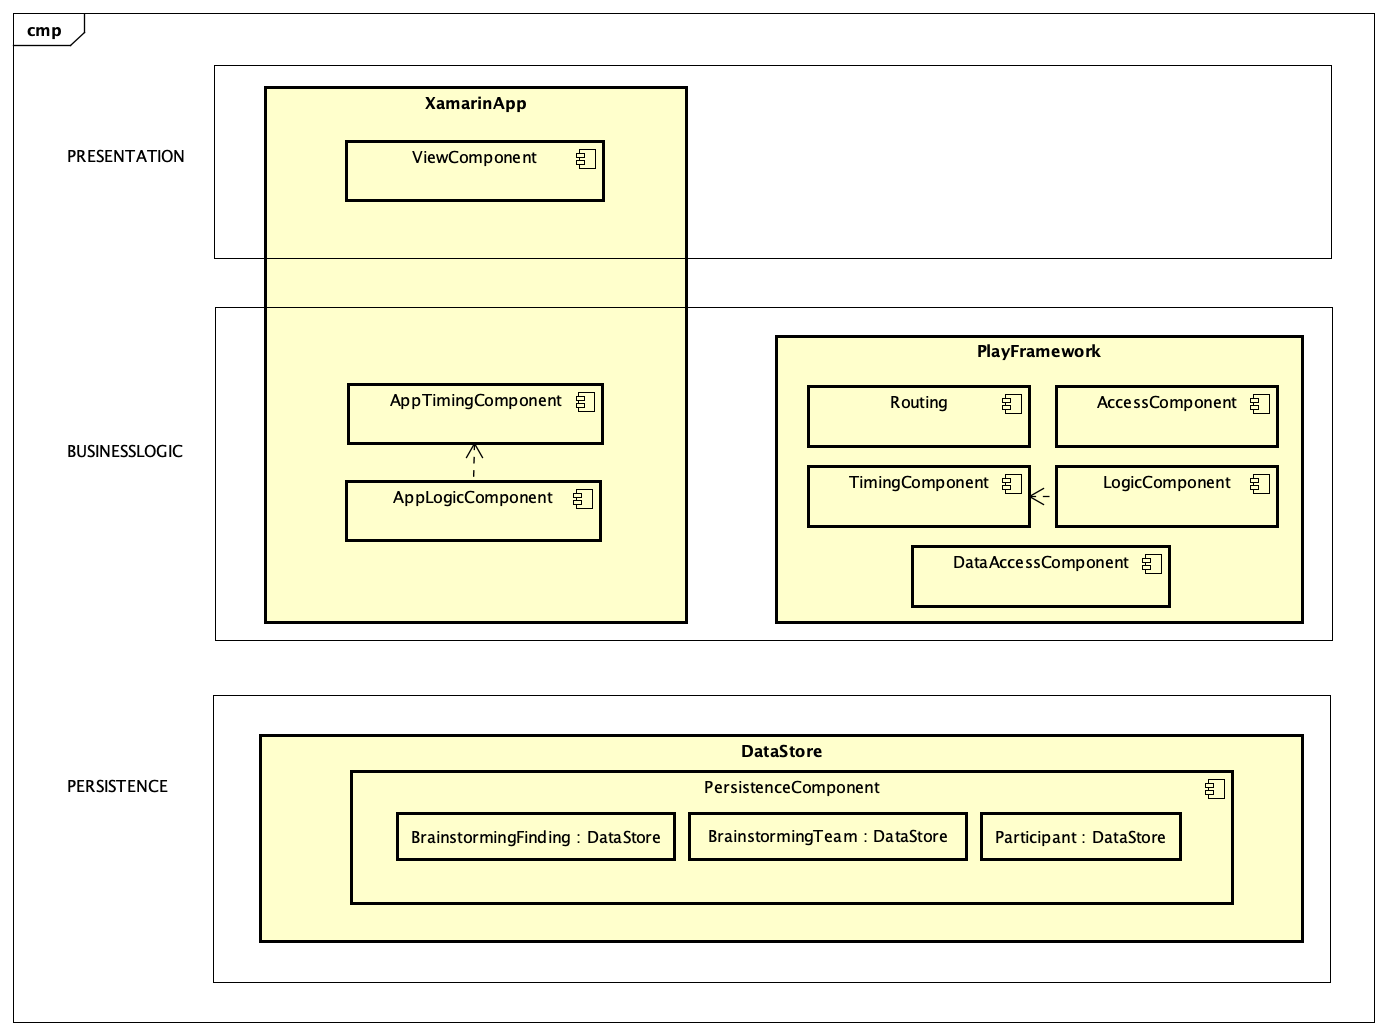
\includegraphics[width=1\linewidth]{img/architektur/CD_Methode635}
	\caption{Logische Architektur BrainingOutOfBox}
	\label{fig:architektur-methode635}
\end{figure}

\paragraph*{Komponenten}

\begin{description}[leftmargin=!,labelwidth=\widthof{\bfseries DataAccessComponent}]
	\item[ViewComponent] Die einzelnen View-Komponenten der Xamarin App sind für das korrekte Anzeigen der Informationen verantwortlich. Sie definieren im wesentlichen das Aussehen der Applikation.
	\item[AppTimingComponent] Die Xamarin App hält in der logischen Schicht eine Timing-Komponente, welche dafür sorgt, dass ein \textit{BrainstormingFinding} nach Ablauf der Zeit abgesendet wird.
	\item[AppLogicComponent] Die Logik-Komponente der Xamarin App regelt weitere Logik, wie z.B. den Zugriff auf das PlayFramework.
	\item[AccessComponent] Die Access-Komponente auf dem PlayFramework regelt den Zugriff mittels JWT-Token\cite{jwt}.
	\item[Routing] Die Routing-Komponente sorgt anhand des URLs für das Aufrufen der korrekten Funktion.
	\item[TimingComponent] Wie die Xamarin App hält auch das PlayFramework eine Timing-Komponente, um den Zustand der Zeit halten zu können.
	\item[LogicComponent] In der Logik-Komponente werden die eigentlichen Funktionen geschrieben. Hier ist auch die Logik für den Austausch der Blätter untergebracht.
	\item[DataAccessComponent] Mit DataAccess-Komponente kann auf die Daten zugegriffen werden.
	\item[PersistenceComponent] Die Persistence-Komponente ist für das Speichern der Daten verantwortlich.
\end{description}


\subsubsection{Deployment}
Wie in der Abbildung \ref{fig:deployment-methode635} zu sehen ist, besteht unser System aus zwei physikalischen Geräten. Das ist zum einen der client und zum anderen der backendNode. Diese beinhalten jeweils sogenannte \textit{DeploymentUnits} (DU). 

Beim client handelt es sich im Grunde um das Smartphone des jeweiligen Benutzers. Auf seinem Smartphone läuft dann die Xamarin App, welche wiederum die appPresentationLayerDU und die appBusinessLogicLayerDU hält.

Der backendNode ist ein Ubuntu 18.04 auf dem ein Java Runtime Environment (JRE) installiert ist. Innerhalb der JRE läuft das PlayFramework, in dem wiederum die businessLogicLayerDU läuft.

Zudem ist auf dem backendNode ein MongoDB Service installiert, welche  die persistenceLogicLayerDU beinhaltet.

\begin{figure}[h]
	\centering
	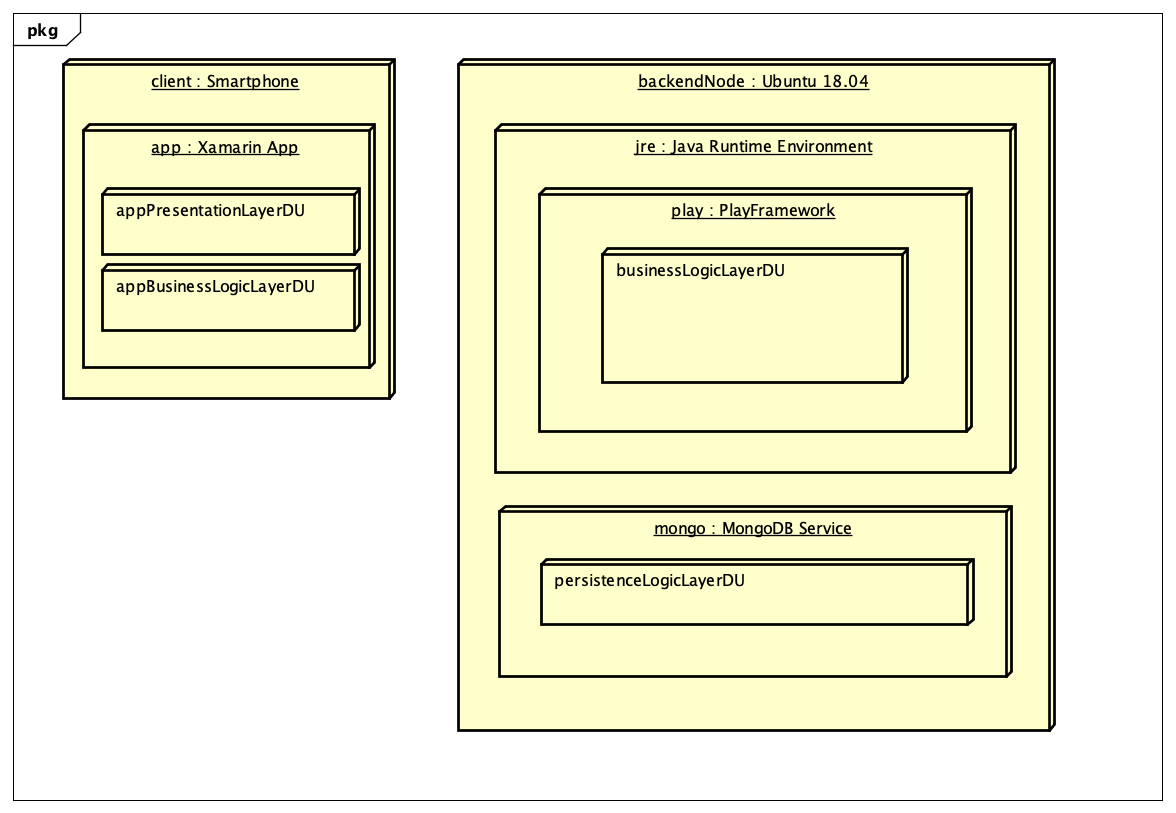
\includegraphics[width=1\linewidth]{img/deployment/DD_Methode635}
	\caption{Deploymentdiagramm BrainingOutOfBox}
	\label{fig:deployment-methode635}
\end{figure}

\paragraph*{Komponenten}

\begin{description}[leftmargin=!,labelwidth=\widthof{\bfseries appBusinessLogicLayerDU}]
	\item[businessLogicLayerDU] Die businessLogicLayerDU enthält alle Komponenten, welche in Abbildung \ref{fig:architektur-methode635} in der logischen Schicht im PlayFramework eingezeichnet sind.
	\item[persistenceLogicLayerDU] Die persistenceLogicLayerDU enthält alle Komponenten, welche in Abbildung \ref{fig:architektur-methode635} in der persistence Schicht eingezeichnet sind.
	\item[appPresentationLayerDU] Die appPresentationLayerDU enthält alle Komponenten, welche in Abbildung \ref{fig:architektur-methode635} in der Präsentationsschicht eingezeichnet sind.
	\item[appBusinessLogicLayerDU] Die appBusinessLogicLayerDU enthält alle Komponenten, welche in Abbildung \ref{fig:architektur-methode635} in der logischen Schicht in der Xamarin App eingezeichnet sind.
\end{description}
